\documentclass[10pt]{article}
\usepackage[utf8]{inputenc}
\usepackage[T1]{fontenc}
\usepackage{amsmath}
\usepackage{amsfonts}
\usepackage{amssymb}
\usepackage[version=4]{mhchem}
\usepackage{stmaryrd}
\usepackage{graphicx}
\usepackage[export]{adjustbox}
\graphicspath{ {./images/} }
\usepackage{hyperref}
\hypersetup{colorlinks=true, linkcolor=blue, filecolor=magenta, urlcolor=cyan,}
\urlstyle{same}

\title{Singular Value Decomposition: Applications to Image Processing }

\author{Elizabeth A. Compton and Stacey L. Ernstberger, PhD\\
Faculty Mentor: Stacey L. Ernstberger, PhD\\
Mathematics}
\date{}


\begin{document}
\maketitle


\begin{abstract}
Digital images require large amounts of memory, and often we would like to reduce the required memory storage and still retain as much of the image quality as possible. We can consider using the singular value decomposition (SVD) to manipulate these large sets of data, which will allow us to identify the components of the image which contribute the least to overall image quality. In this paper we explore the SVD in general as well as how computing the SVD and removing the singular values can reduce the size of stored images.
\end{abstract}

\section*{Introduction}
When we consider a digital screen, we rarely think about the composition of the images that we are viewing. A screen that displays in color actually has a separate saturation scale of 0 to 255 for red, green, and blue per pixel. If we consider only grayscale, there is a saturation scale of 0 to 255 per pixel [2]. Thus, images can be interpreted as a matrix with pixels represented as individual numerical entries. Rows and columns of a matrix hold the position of the pixel, and each value in the matrix represent the corresponding saturation level. These components can ultimately result in a large amount of memory used to produce a single image. For instance, if we were to save a $100 \times 100$ image in grayscale, there would be 10,000 different pixel values stored. We would like to address a way in which computers can save images without taking up such large amounts of memory.

We consider using the method of Singular Value Decomposition to compress the size of the saturation matrices, retaining the most important components, to save an image using less memory while also retaining the image quality.

\section*{Singular Value Decomposition}
The process of Singular Value Decomposition (SVD) involves breaking down a matrix $A$ into the form $A=U \Sigma V^{T}$. This computation allows us to retain the important singular values that the image requires while also releasing the values that are not as necessary in retaining the quality of the image. The singular values of an $m \times n$ matrix $A$ are the square roots of the eigenvalues of the $n \times n$ matrix $A^{T}$ $A$, which are typically organized by magnitude in decreasing order [4]. The Singular Value Decomposition is so named due\\
to the singular values that are identified and isolated from matrix $A$.

\section*{How to Compute the SVD of a Matrix}
We will rewrite an $m \times n$ matrix $A$ in the form $A=U \Sigma V^{T}$, where $U$ is an $m \times m$ matrix orthonormal columns, $\Sigma$ is an $m \times n$ matrix with singular values on the main diagonal, and $V$ is an $n \times n$ matrix with orthonormal columns. $V^{T}$ is the transpose of matrix $V$, which is found by exchanging the rows and the columns of the matrix.

Note: If two column vectors form an orthonormal set, it means that the inner product of the columns with each other is 0 , and the inner product of any column with itself is 1 . Hence, any matrix $B$ that has orthonormal columns has the property $B^{T} B=I=B B^{T}$, where $I$ is the identity matrix.

Before we apply the SVD to image processing, we will first demonstrate the method using a small ( $2 \times 3$ ) matrix $A$ :

$$
A=\left[\begin{array}{lll}
3 & 2 & 1 \\
2 & 1 & 4
\end{array}\right]
$$

and then follow a step-by-step process to rewrite the matrix $A$ in the separated form $U \Sigma V^{T}$.

\section*{Step 1: Form $A^{T} A$}
We begin by forming $A^{T} A$ for our given matrix $A$ by performing basic matrix multiplication as follows:

$$
A^{T} A=\left[\begin{array}{ll}
3 & 2 \\
2 & 1 \\
1 & 4
\end{array}\right]\left[\begin{array}{lll}
3 & 2 & 1 \\
2 & 1 & 4
\end{array}\right]=\left[\begin{array}{ccc}
13 & 8 & 11 \\
8 & 5 & 6 \\
11 & 6 & 17
\end{array}\right] .
$$

This process will result in a square matrix of dimension $n \times n$ with non-negative values, and here we can see that we have only non-negative values in our resulting $3 \times 3$ matrix.

\section*{Step 2: Determine the eigenvalues of $A^{T} A$}
In order to determine the eigenvalues of $A^{T} A$, we need to compute the determinant of the matrix $A^{T} A-\lambda I$. In general, we compute the determinant of a $3 \times 3$ matrix in the following way:

$$
\begin{aligned}
\left|\begin{array}{lll}
a & b & c \\
d & e & f \\
h & i & j
\end{array}\right| & =a\left|\begin{array}{ll}
e & f \\
h & i
\end{array}\right|-d\left|\begin{array}{ll}
b & c \\
h & i
\end{array}\right|+g\left|\begin{array}{ll}
b & c \\
e & f
\end{array}\right| \\
& =a(e i-f h)+d(b i-h c)+g(b f-c e) .
\end{aligned}
$$

We could clearly extend this computation to an $n \times n$ matrix as needed. For our example, we compute the determinant of $A^{T} A-\lambda I$ which is:

$$
\begin{aligned}
{\left[\begin{array}{ccc}
13 & 8 & 11 \\
8 & 5 & 6 \\
11 & 6 & 17
\end{array}\right]-\lambda\left[\begin{array}{lll}
1 & 0 & 0 \\
0 & 1 & 0 \\
0 & 0 & 1
\end{array}\right] } & \left.=\left\lvert\, \begin{array}{ccc}
13-\lambda & 8 & 11 \\
8 & 5-\lambda & 6 \\
11 & 6 & 17-\lambda
\end{array}\right.\right] \\
& =(13-\lambda)[(5-\lambda)(17-\lambda)-(6)(6)]-8[(8)(17-\lambda)-(11)(6)]+ \\
& 11[(8)(6)-(11)(5-\lambda)] \\
& =\lambda^{3}+35 \lambda^{2}+150 \lambda \\
& =\lambda(\lambda-5)(\lambda-30) .
\end{aligned}
$$

By setting this determinant equal to zero, we solve what is called the characteristic equation for $\lambda$, and here we see that $\lambda$ $=0,5,30$. We reorder the eigenvalues in decreasing magnitude, so that: $\lambda_{1}=30, \lambda_{2}=5$, and $\lambda_{3}=0$.

\section*{Step 3: Form the matrix $V^{T}$}
Once we have determined the eigenvalues, we then compute the corresponding eigenvectors and normalize them to produce the matrix $V$. In general, we compute eigenvectors by using the matrix $A^{T} A-\lambda I$ and simplify the matrix for each eigenvalue. For example, for $\lambda_{1}=30$ we have:\\
$A^{T} A-\lambda_{1} I=\left[\begin{array}{ccc}13-30 & 8 & 11 \\ 8 & 5-30 & 6 \\ 11 & 6 & 17-30\end{array}\right]=\left[\begin{array}{ccc}-17 & 8 & 11 \\ 8 & -25 & 6 \\ 11 & 6 & -13\end{array}\right]$.

We then solve the homogeneous equation $\left(A^{T} A-\lambda I\right) \vec{x}_{1}=\overrightarrow{0}$ to obtain the eigenvector $\vec{x}_{1}$, which here results in:

$$
\vec{x}_{1}=\left[\begin{array}{c}
-\frac{323}{361} \\
-\frac{190}{361} \\
1
\end{array}\right]
$$

We then normalize the eigenvector by dividing by its magnitude to form a new vector:

$$
\vec{v}_{1}=\frac{\vec{x}_{1}}{\left|\vec{x}_{1}\right|}=\frac{1}{\sqrt{\frac{750}{361}}}\left[\begin{array}{c}
-\frac{323}{361} \\
-\frac{190}{361} \\
1
\end{array}\right]=\left[\begin{array}{c}
\frac{-17}{5 \sqrt{30}} \\
\frac{-10}{5 \sqrt{30}} \\
\frac{19}{5 \sqrt{30}}
\end{array}\right]
$$

We do this for each eigenvalue to produce a full set of eigenvectors that we will use to form the matrix $V$. For our example,

$$
V=\left[\begin{array}{lll}
\vec{v}_{1} & \vec{v}_{2} & \vec{v}_{3}
\end{array}\right]=\left[\begin{array}{ccc}
\frac{-17}{5 \sqrt{30}} & \frac{-6}{5 \sqrt{5}} & \frac{7}{5 \sqrt{6}} \\
\frac{-10}{5 \sqrt{30}} & \frac{-5}{5 \sqrt{5}} & \frac{-2}{\sqrt{6}} \\
\frac{19}{5 \sqrt{30}} & \frac{8}{5 \sqrt{5}} & \frac{-1}{5 \sqrt{6}}
\end{array}\right] .
$$

The matrix $V^{T}$ can be easily obtained from $V$, which results in the columns interchanging with the corresponding rows. Thus, we have the resulting matrix

$$
V^{T}=\left[\begin{array}{ccc}
\frac{-17}{5 \sqrt{30}} & \frac{-10}{5 \sqrt{30}} & \frac{19}{5 \sqrt{30}} \\
\frac{-6}{5 \sqrt{5}} & \frac{-5}{5 \sqrt{5}} & \frac{8}{5 \sqrt{5}} \\
\frac{7}{5 \sqrt{6}} & \frac{-2}{\sqrt{6}} & \frac{-1}{5 \sqrt{6}}
\end{array}\right]
$$

\section*{Step 4: Form the matrix $\Sigma$}
To determine the matrix $\Sigma$, we list the nonzero singular values, $\sigma_{i}$, in decreasing magnitude down the main diagonal of $\Sigma$, where $\sigma_{i}=\sqrt{\lambda_{i}}$. Then we add any additional rows and columns of zeros as needed to retain the original dimension of $A$ in $\Sigma$. In our example we have three singular values: $\sqrt{3} 0$, $\sqrt{5}$, and 0 . We only need to retain the non-zero values, and hence we form the matrix

$$
\Sigma=\left[\begin{array}{ccc}
\sqrt{30} & 0 & 0 \\
0 & \sqrt{5} & 0
\end{array}\right] .
$$

Note that $\Sigma$ has the same dimension as our original matrix $A$.

\section*{Step 5: Form the matrix $U$}
We form the matrix $U$ by considering our modified form $A=U \Sigma V^{T}$, and isolating each column of $U$. Because of the diagonal nature of $\Sigma$, this results in

$$
\vec{u}_{i}=\frac{1}{\sigma_{i}} A \vec{v}_{i}
$$

for each of the singular values. We have two singular values in our example, and we use them to form the following vectors:\\
$\vec{u}_{1}=\frac{1}{\sqrt{30}}\left[\begin{array}{lll}3 & 2 & 1 \\ 2 & 1 & 4\end{array}\right]\left[\begin{array}{c}\frac{-17}{5 \sqrt{30}} \\ \frac{-10}{5 \sqrt{30}} \\ \frac{19}{5 \sqrt{30}}\end{array}\right]=\left[\begin{array}{c}\frac{3}{5} \\ \frac{4}{5}\end{array}\right] \quad$ and $\quad \vec{u}_{2}=\frac{1}{\sqrt{5}}\left[\begin{array}{lll}3 & 2 & 1 \\ 2 & 1 & 4\end{array}\right]\left[\begin{array}{c}\frac{-6}{5 \sqrt{5}} \\ \frac{-5}{5 \sqrt{5}} \\ \frac{8}{5 \sqrt{5}}\end{array}\right]=\left[\begin{array}{c}4 \\ 5 \\ -\frac{3}{5}\end{array}\right]$.\\
We then combine these column vectors to form the matrix:

$$
U=\left[\begin{array}{ll}
\vec{u}_{1} & \vec{u}_{2}
\end{array}\right]=\left[\begin{array}{cc}
\frac{3}{5} & \frac{4}{5} \\
\frac{4}{5} & -\frac{3}{5}
\end{array}\right] .
$$

Note that the columns of $U$ are again orthonormal.\\
Step 6: Rewrite matrix $\boldsymbol{A}$ as $U \Sigma V^{T}$\\
Finally, we rewrite $A$ using the equation $A=U \Sigma V^{T}$

$$
A=\left[\begin{array}{cc}
\frac{3}{5} & \frac{4}{5} \\
\frac{4}{5} & -\frac{3}{5}
\end{array}\right]\left[\begin{array}{ccc}
\sqrt{30} & 0 & 0 \\
0 & \sqrt{5} & 0
\end{array}\right]\left[\begin{array}{ccc}
\frac{-17}{5 \sqrt{30}} & \frac{-10}{5 \sqrt{30}} & \frac{19}{5 \sqrt{30}} \\
\frac{-6}{5 \sqrt{5}} & \frac{-5}{5 \sqrt{5}} & \frac{8}{5 \sqrt{5}} \\
\frac{7}{5 \sqrt{6}} & \frac{-2}{\sqrt{6}} & \frac{-1}{5 \sqrt{6}}
\end{array}\right]
$$

This decomposition provides a broken-down form of the matrix A that has isolated the most important components from our original matrix. This returns a modification of our original matrix A in which the components are smaller in size, thus reducing the memory requirement in storing the information.

\section*{Applications to Image Processing}
The process of Singular Value Decomposition can be used in many applications, including watermarking an image, computing weighted least squares, and optimal prediction. Here we will consider how this process could be used to produce reduced image sizes. We begin by\\
understanding that large images are formed by correspondingly large matrices, hence requiring a sizable amount of memory to store the image. By rewriting the image in its broken-down form and removing the smaller singular values, we can form smaller matrices which would in turn require less memory storage. We would lose some refinement with each loss of a singular value, but overall, we would retain the overall image features.

\section*{Implementation in Grayscale}
In MATLAB, we use and modify existing code from Dr. Brady Matthews' paper "Image Compression using Singular Value Decomposition" to load an image, isolate the corresponding saturation matrix, and then modify the matrix based on its singular values [2]. As an example, we use a high-contrast grayscale image of a feather seen in Figure 1.\\
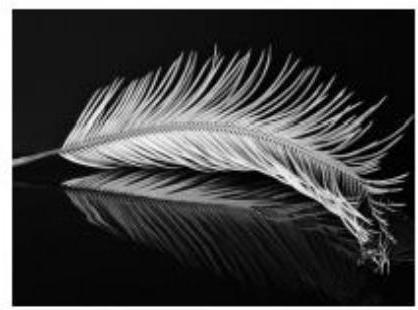
\includegraphics[max width=\textwidth, center]{2025_04_09_7d70d965b908bc4c1892g-3}

Figure 1: Original high-contrast grayscale image [5]\\
We consider the individual saturation levels of each pixel in the original image as the numerical entries in a matrix. We compute the SVD of that matrix and remove the singular values (from smallest to largest), converting the modified matrices (with removed values) back into a series of images. This process of decomposition can reduce the image storage size without losing the quality needed to fully represent the image.

In Figure 2 we can see that as more singular values are included in the image matrix, the clarity of the image improves.\\
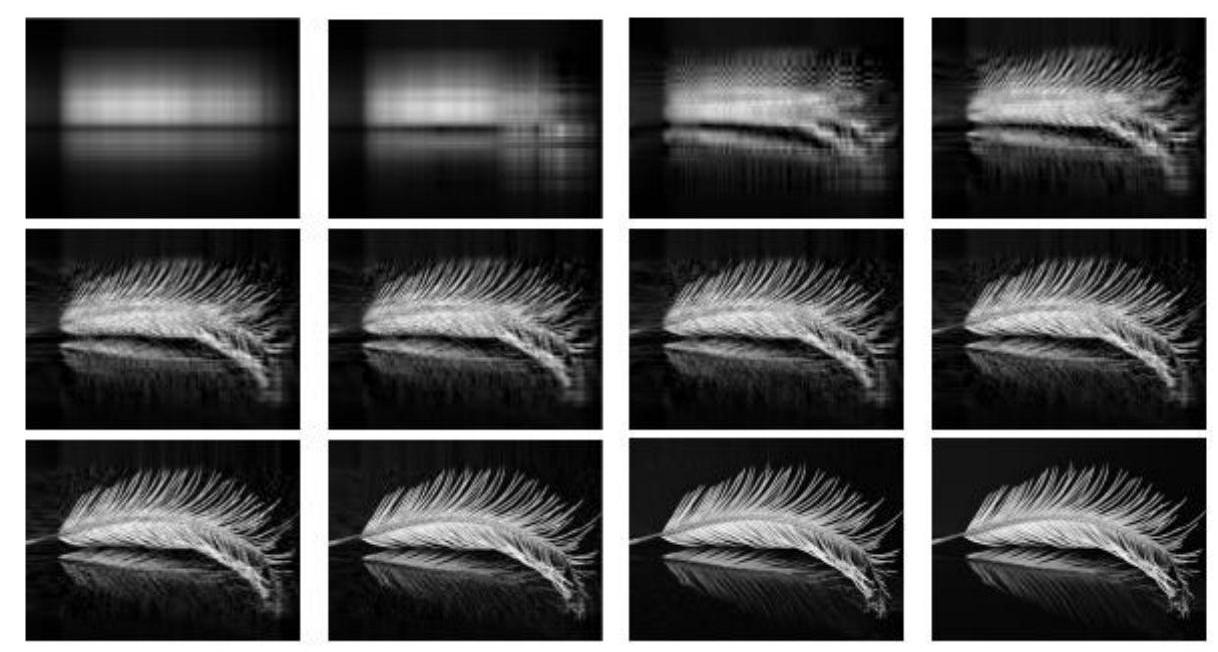
\includegraphics[max width=\textwidth, center]{2025_04_09_7d70d965b908bc4c1892g-3(1)}

Figure 2: Number of Singular Values: $\{1,2,5,10\}\{15,18,24,30\}\{35,60,120,680\}$\\
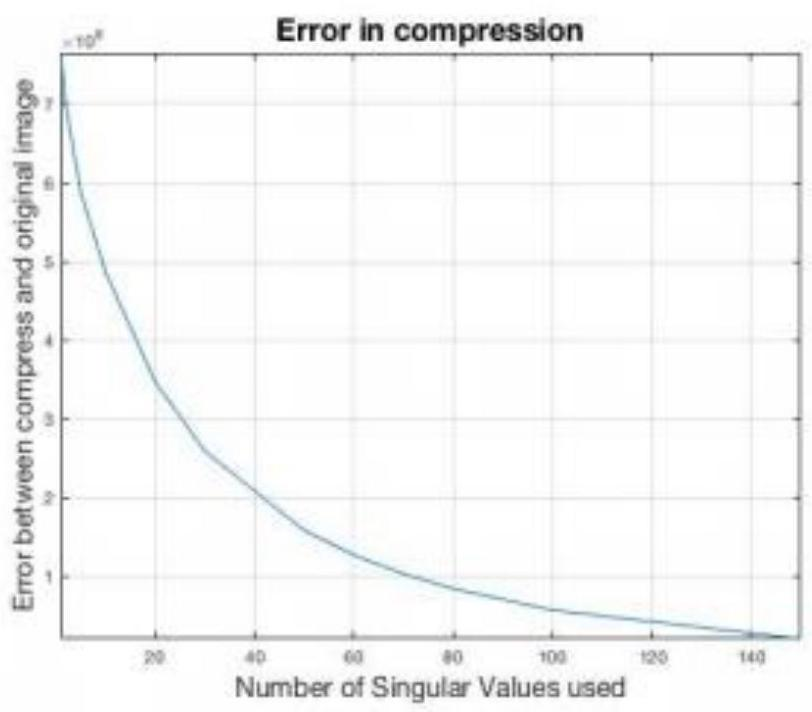
\includegraphics[max width=\textwidth, center]{2025_04_09_7d70d965b908bc4c1892g-4(1)}

Figure 3: Error in compression when applied to the grayscale feather image.\\[0pt]
The original image has approximately 680 singular values, but we were able to see a close resemblance to the original image using only 120 singular values [5]. The amount of storage space is not as significant in our example here as it would be in practice, because of our emphasis on image clarity. Our current process is to compress while still retaining the original number of pixels in order to show the details of the loss of image quality. In practice, we would see a more significant change in storage of an image if we allowed the overall image size (the number of pixels) to reduce as we removed the small singular values. For example, we can see this relation in photos that have been initially taken on a phone and then sent via text, often appear more course since they have been compressed along the way.

In Figure 3, we see the amount of error in saturation level differences from the original image. We observe the positive concavity of the error curve, which indicates that as the error decreases, the rate of change of the error loss also\\
decreases. This means that the rate of change of the error loss is less significant as more singular values are used. Here we see that the sharp negative slope that happens prior to approximately 20 singular values corresponds with the blurry images that were unrecognizable in Figure 2. As we continue to reintroduce a greater number of singular values, we can see the quality of the image increase, but we can see almost as many details with 30 values as we could with 680.

\section*{Removing Larger Singular Values}
We now extend this concept to the initial removal of larger singular values from an image instead of smaller singular values. We intuitively know that this would not be useful in retaining image quality but are curious as to the extreme nature of the image without the largest singular values. Originally the MATLAB code computed the SVD of the matrix of the image and removed the singular values (from smallest to largest). Then this process would convert the modified matrices (with removed values) back into images as shown in Figure 2. Through careful manipulation we redeveloped the code to build a series of matrices by instead starting with only the smallest values. Then these matrices were converted into images that have the same number of pixels as in the original image. This visualization is shown in Figure 4.

Through careful evaluation we are able to observe the same trend from Figure 2 that as more singular values are included in the image, the corresponding image clarity increases. However, where in the prior example we only required a few large singular values to produce a reasonable image, here we see that we need a very large number of singular values to produce a similar quality image since we are only using the smaller singular values first. In Figure 4 we can see that there are nearly 625 singular values needed for anything visible upon the black landscape. As we reintroduce\\
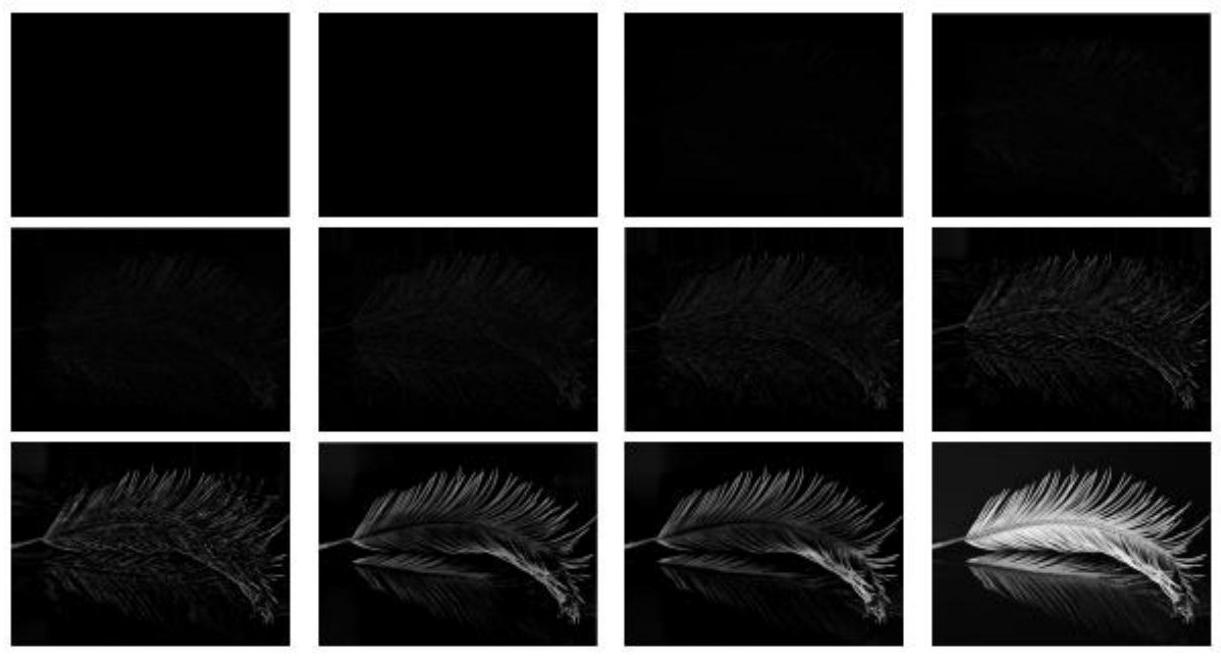
\includegraphics[max width=\textwidth, center]{2025_04_09_7d70d965b908bc4c1892g-4}

Figure 4: Number of Singular Values: $\{1,250,500,550\}\{575,600,625,650\}\{665,678,679,680\}$\\
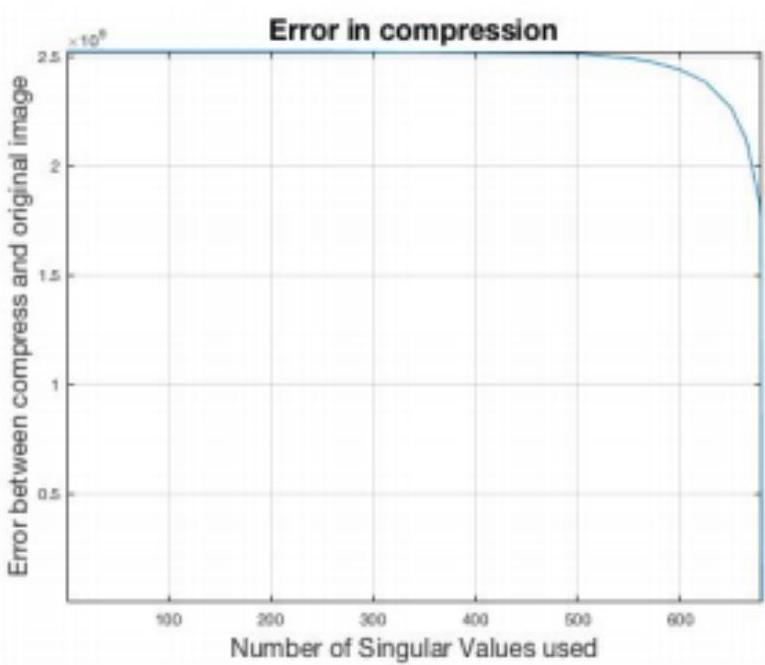
\includegraphics[max width=\textwidth, center]{2025_04_09_7d70d965b908bc4c1892g-5(2)}

Figure 5: Error using this particular model.\\
the larger singular values, the corresponding quality of the images drastically increase.

We again view the error curve which displays a numerical representation for the difference between an approximated matrix with fewer singular values and our original matrix. The jump that occurs from the incorporation of a higher number of singular values is represented in Figure 5. The negative concavity of this error curve becomes visible as the number of singular values are reintroduced. There appears to be a point of when there are greater than approximately 550 singular values the error between the compress and original image decreases. This error curve is supported though the visual representation within Figure 4, that the image quality improves in a significant manner as the larger singular values are reincorporated.

Through this investigation of singular values, we have observed the significance of the largest singular value, and we now isolate the images using this value alone in Figure 6. This figure shows the representation of the largest singular value and how it contributes to the overall image quality. We note that there is a significant difference when we remove just the largest singular value, as it contributed the most to the information contained in the original image matrix that corresponded to our grayscale image.

\section*{Implementation to full color images}
We have been able to observe that the process of SVD can be used to compress images to conserve storage space by removing the singular values that contribute the least to the information contained in the image matrix. Thus far we have only demonstrated compression for a grayscale image, but we will now expand this process to full color images. For this simulation we will choose a full color detailed image that celebrates our favorite mathematical holiday, Pi Day, as seen in Figure 7.\\

\includegraphics[max width=\textwidth, center]{2025_04_09_7d70d965b908bc4c1892g-5}

Figure 7: Original Pi Day image [6]\\
Recall that each pixel in full color image has color saturation representation values of 0 to 255 for red, green, and blue. This adds complexity to the image, which requires a greater amount of storage space used to save a particular image. By showing the representation of each color relative to the full color image, we are able to see the amount of contribution each color has to each pixel as shown in Figure 8. In order to implement the SVD process we will have to first separate the full color image into its red, green, and blue layers, as each of these three colors has its own matrix of information for the image. We will remove the smallest singular values from each of the color matrices, and then we will reconstruct the full color image using the modified color matrices.

This decomposition is shown in a simplistic form in Figure 8. As we compute the SVD and only reintroduce specific singular values, we see the image quality increase within Figure 9. With only one singular value, there is very little we can recognize from the original image. As singular values are reintroduced, we are able to see the image more clearly to be a celebration of Pi Day. For this particular image, this compression process was able to save a considerable\\
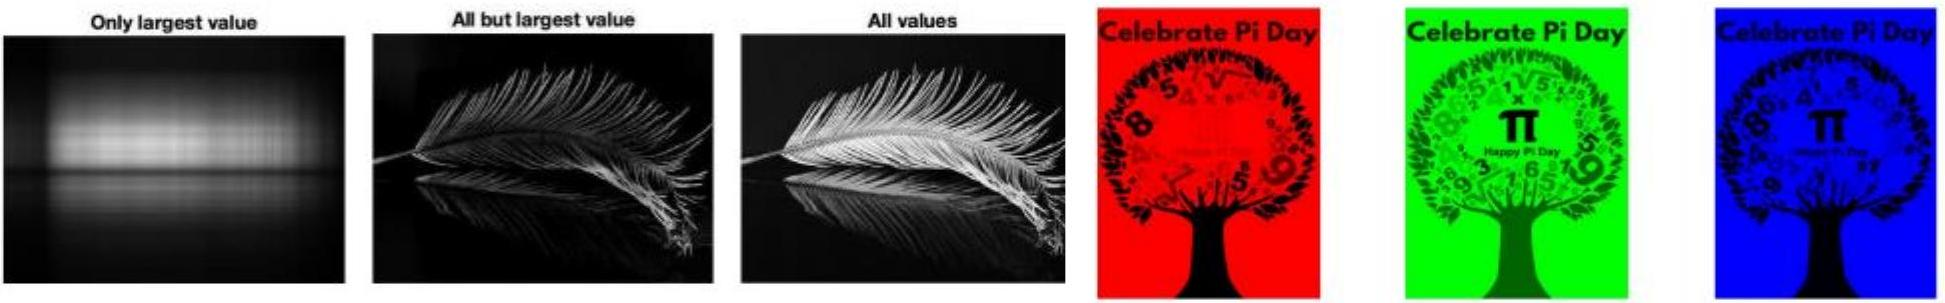
\includegraphics[max width=\textwidth, center]{2025_04_09_7d70d965b908bc4c1892g-5(1)}

Figure 6: Importance of the Largest Singular Value\\
Figure 8: Pi Day image with red, green, and blue saturation layers isolated\\
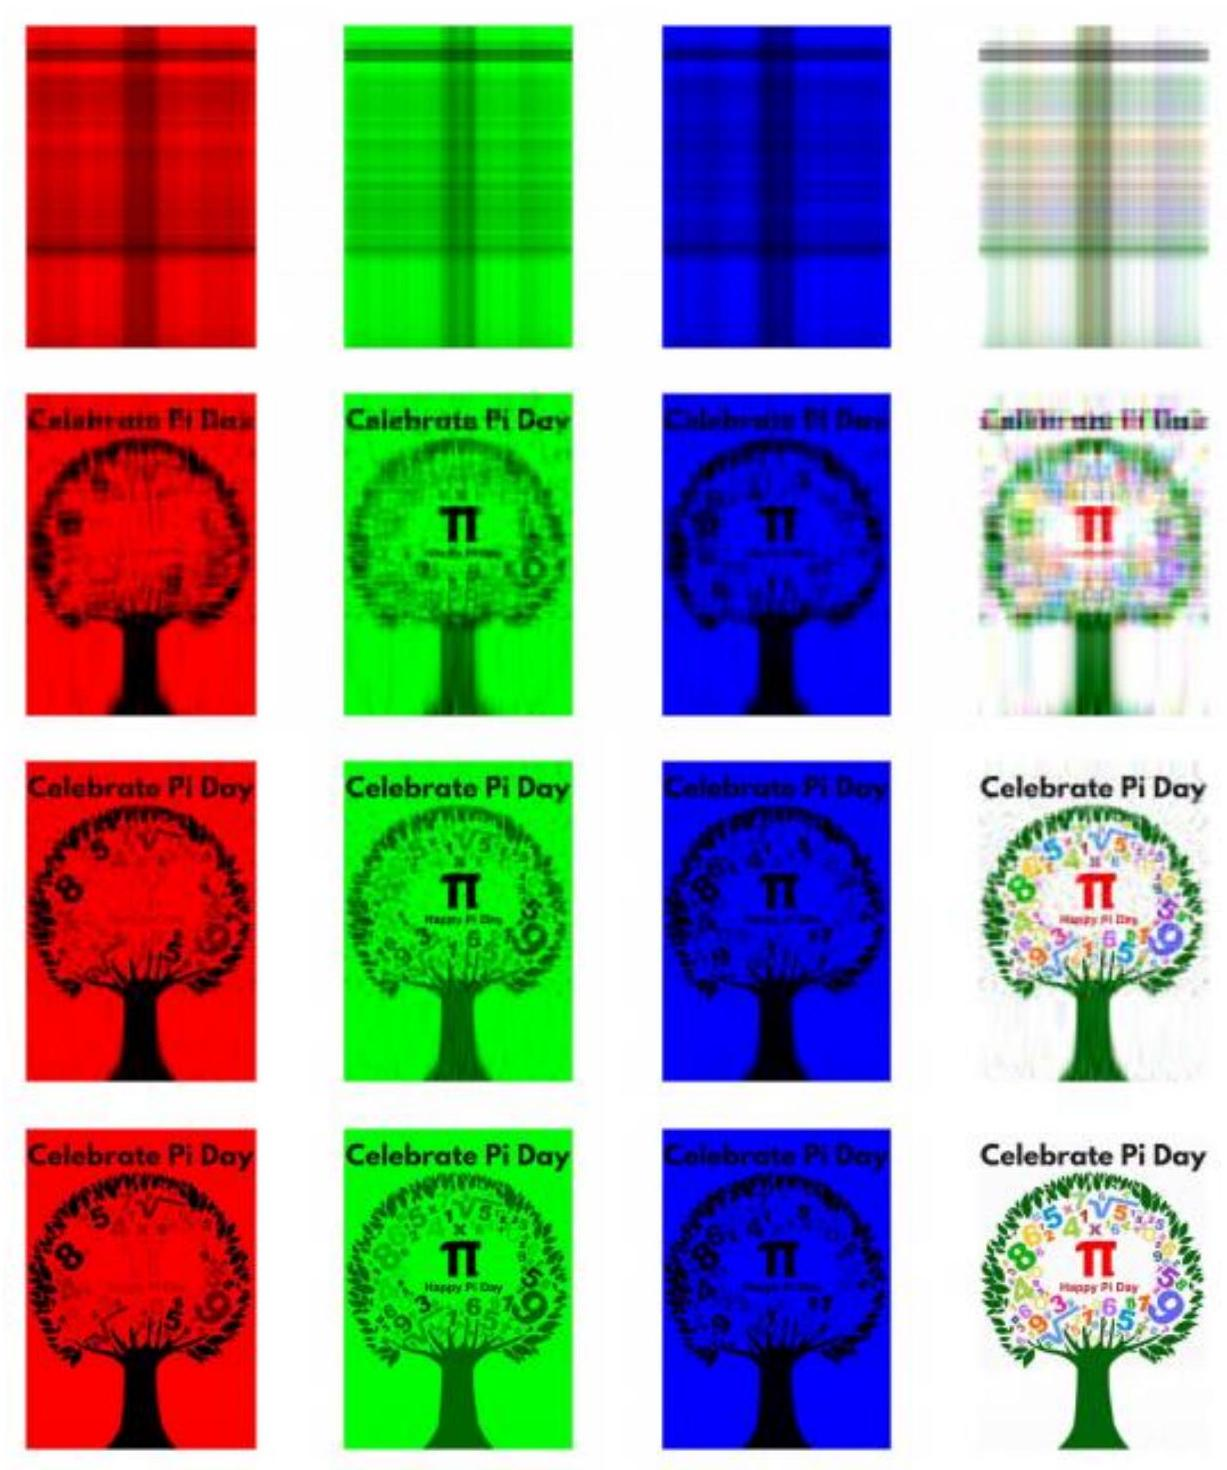
\includegraphics[max width=\textwidth, center]{2025_04_09_7d70d965b908bc4c1892g-6(1)}

Figure 9: Number of singular values per row: $\{1,10,25,100\}$\\
amount of space compared to our grayscale example observed in Figure 2.

The error for full color images is more complex to observe than the error corresponding to a grayscale image, due to the fact that we separated the color image into three separate color saturation matrices. The error curves in Figure 10 represent the accumulated error when comparing each modified color saturation matrix to the corresponding color saturation matrix from the original image. We are again able to notice a considerable change in clarity from the images compressed using a relatively low number of singular values. In addition to the obvious reduction of error with the addition of more singular values, we also observe a noticeable difference between the error curves within each pixel color. This original image in Figure 7 has a considerable amount of green which contributes largely to the image clarity when represented only with the green pixel contribution. In an opposing manner, there is not much representation from the\\
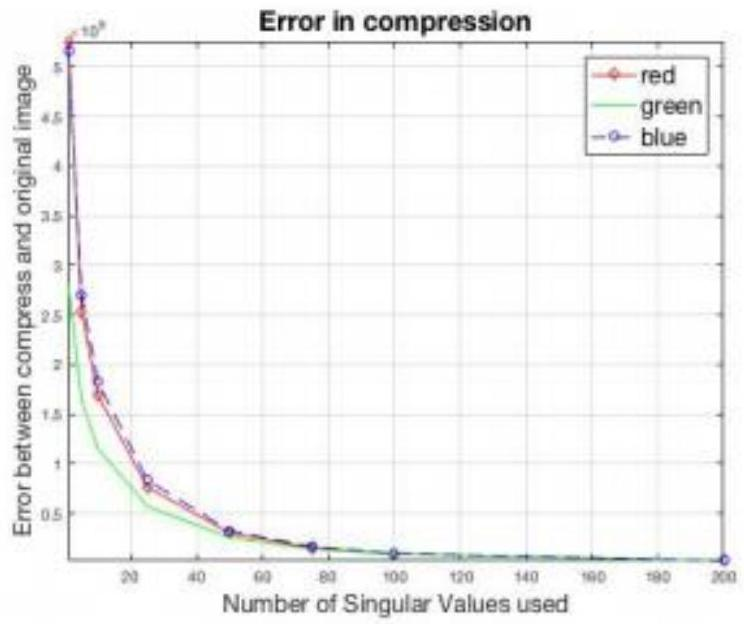
\includegraphics[max width=\textwidth, center]{2025_04_09_7d70d965b908bc4c1892g-6}

Figure 10: Error curves for the red, green, and blue pixel saturation levels from the Pi Day image\\
blue or red pixel saturation layers, and hence in Figure 10 we can see that the error changes more significantly in the green saturation layer than with the other two layers.

We consider our initial challenge of saving storage space using the SVD when applied to image processing, and we note that for this small full color image we were able to see a noticeable difference in storage size. The original image had 574 singular values for each of the color layers, and when we compare this image to the full color image with 100 singular values, we use approximately $50 \%$ of the original storage space. We can see in Figure 11 that they look almost identical when compared side to side, but the storage size and information matrices are much smaller. Recall that for the sake of direct comparison we have retained the original number of pixels in these comparisons, instead of naturally reducing the number of pixels as we removed each unimportant singular value. The corresponding storage size would drastically decrease if we allowed this to occur.\\
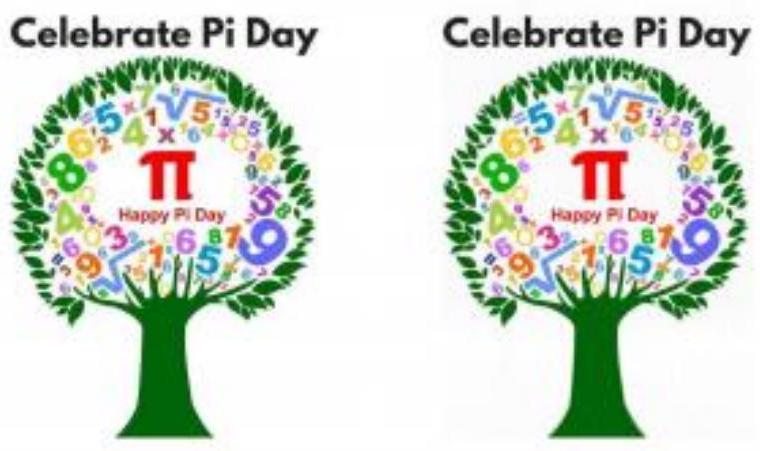
\includegraphics[max width=\textwidth, center]{2025_04_09_7d70d965b908bc4c1892g-7}

Figure 11: Original image and the compressed image

\section*{Conclusions}
By applying the process of Singular Value Decomposition to images by using pixel saturation matrices for grayscale or full color images, we can compress the storage size of an image even while retaining the number of pixels. We have isolated the least important pieces of information that are stored in the images and have removed them methodically,\\
leaving only the most important components of the images. This process of removing the smallest singular values from the saturation matrices allows us to retain as much of the image quality as possible. In the future we can further explore the usefulness when applied to image processing by allowing the image size to decrease when we remove the singular values, which would garner more extensive results in storage size reduction. Beyond this, we can additionally consider applying this method to each frame of a video, potentially resulting in a significant amount of storage size savings as well. These are some of the many ways that the Singular Value Decomposition Method can be helpful when applied to large matrices of information.

\section*{References}
[1] Cao, Lijie. "Singular value decomposition applied to digital image processing." Division of Computing Studies, Arizona State University Polytechnic Campus, Mesa, Arizona State University polytechnic Campus (2006): 1-15.\\[0pt]
[2] Mathews, Brady, "Image Compression using Singular Value Decomposition (SVD)," 2014.\\[0pt]
[3] Ewerbring, L. Magnus, and Franklin T. LUK. "Canonical Correlations and Generalized SVD: Applications and New Algorithms." Advances in Parallel Computing, North-Holland, 27 June 2014.\\[0pt]
[4] Lay, David C., Linear Algebra and its Applications, 3rd updated Edition, 2005.\\[0pt]
[5] Da Costa, Antonio, "Relic of Icarus," ViewBug, \href{https://www.viewbug.com/photo/56748962}{https://www.viewbug.com/photo/56748962}, 2015.\\[0pt]
[6] "Celebrate Pi Day," Clipart Pi Day, \href{https://clipartart.com/categories/clipart-pi-day.html}{https://clipartart.com/categories/clipart-pi-day.html}, 2019.


\end{document}